\subsection{Multi-instance learning}

\subsubsection{Classical}
Multi-instance learning (MIL) is a supervised learning method.
Typically, every instance in a dataset is labelled individually.
However, with MIL, the model receives a bag of instances, $B=\{(x_1,y_1),\ldots,(x_K,y_K)\}$, where $x$ is an instance with label $y$.
Under the standard assumption, the label of a bag is
\begin{align}
    Y(B) &= 1 - \prod_{k}^{K}(1-y_k) \\
         &= \max_k(y_k),
\end{align}
\ie, a bag is positive if at least one instance is positive.

The standard assumption is assymetric: the meaning of the bag label changes if positive and negative labels are swapped.
This assumption might be too restrictive in non-binary problems.

See \cref{fig:classifier} for a schematic overview of a general MIL model.

\begin{figure*}
    \centering
    \includesvg[width=\linewidth]{pediatric-brain-tumours/images/classifier.svg}
    \caption[Multi-instance learning classification]{
        Extracted features (tile features in this work) are presented to a multi-layer perceptron (MLP) with learnable weights.
        The first MLP outputs an aggregate that summarizes all input features.
        The aggregate is used as input to a classifier MLP with learnable weights that outputs a prediction.
        Weights are updated based on pre-defined loss between prediction and target.
    }
    \label{fig:classifier}
\end{figure*}

\todo[noline]{describe need for newer MIL methods}

\subsubsection{Attention-based MIL pooling}
To overcome the restrictive nature of maximum pooling, \textcite{Ilse2018} propose DeepMIL and use a adaptive weighted average of instances.
This weighted average includes learnable weights in an attention-based manner.
Let $H=\{\vec{h}_1, \ldots, \vec{h}_K\}$ be a bag of $K$ embeddings.
The weighted average of $H$ is
\begin{equation}
    \vec{z}=\sum_{k=1}^{K}a_k\vec{h}_k,
\end{equation}
where
\begin{equation}
    a_k = \frac{\exp\left[\mathbf{w}^T \tanh (\mathbf{V}\vec{h}_k^T)\right]}{\sum_{j=1}^{K}\exp\left[\mathbf{w}^T \tanh (\mathbf{V}\vec{h}_k^T)\right]},
\end{equation}\todo[noline]{add bias terms}
where $\mathbf{w} \in \mathbb{R}^{L \times 1}$ and $\mathbf{V}\in \mathbb{R}^{L \times M}$ are the learnable parameters.
The denominator ensures the weights sum to 1.
$\vec{z}$ is further processed in an MLP for classification.

The weights allow to distinguish interesting instances from uninteresting ones, see \cref{fig:explainer}
High weights should be assigned to instances that are likely to have a positive label.
This is particularly important for pathology studies.
The attention weights of specific instances (\eg, patches in an image) explain how the model comes to its diagnosis prediction that can be compared with the doctor's diagnosis.

\begin{figure*}
    \centering
    \includesvg[width=\linewidth]{pediatric-brain-tumours/images/explainer.svg}
    \caption[Tile importances]{
        Visualizing tile importances.
        The attention weights resulting from VarMIL are min-max-normalized and multiplied with their corresponding tile.
        The output is an attention weighted image with bright parts relating to high attention and dark parts relating to low attention.
        Note that dark tiles can still have high attentions if the original image contains dark patches with useful information.
    }
    \label{fig:explainer}
\end{figure*}

\subsubsection{Variance MIL pooling}\label{subsubsection:theory_varmil}
Learning weights just for a weighted average discards any interinstance information, while that might be important for the bag prediction.
Variance MIL (VarMIL) by \textcite{Schirris2022} propose to add a learned attention-weighted variance,
\begin{equation}
    \boldsymbol{\sigma} = \frac{K}{K - 1} \sum_{k=1}^{K}a_k\left(\vec{h}_k-\vec{z}\right)^2.
\end{equation}
In a clinical setting, this variance can model \eg the intratumour heterogeneity or tumour border shape.
The weighted average and variance are concatenated in a single vector, such that
\begin{equation}
    \hat{\vec{z}} =
    \begin{pmatrix}
        \vec{z} \\
        \boldsymbol{\sigma}    
    \end{pmatrix}.
\end{equation}

\subsubsection{Clinical Context MIL}
Clinical contexts such as locations of tumour resections are important for clinical decisions by pathologists.
For example, medulloblastoma is mostly found in the fourth ventricle or cerebellar parenchyma.\todo{https://pubmed.ncbi.nlm.nih.gov/26336203/}
This information along with the attention weighted tiles (see \cref{subsubsection:theory_varmil}) may lead to better performance.
As pathologists also have access to this information, it is reasonable for an AI model to use the same available information.

In this work, Clinical Context MIL (CCMIL) is proposed.
CCMIL builds on VarMIL, with the addition of clinical information as input to the classification layer.
The clinical information is presented as a string of characters, a sentence, which can be anything clinically relevant.
The sentence is condensed to a $H\times1$-dimensional text embedding.
The embedding is concatenated to the output of the MIL aggregate, such that
\begin{align}
    \tilde{\vec{z}} =
    \begin{pmatrix}
        \hat{\vec{z}} \\
        \boldsymbol{\mathcal{C}}
    \end{pmatrix},
\end{align}
where $\boldsymbol{\mathcal{C}}$ is the clinical context text embedding.
$\tilde{\vec{z}}$ is used as input for the trainable classifier.

The text embedding can be created in various ways~\cite{Khattak2019}.
The most direct way would be to create a list of possible sentences and convert the input text to a one-hot encoded vector, effectively selecting a specific sentence from the vocabulary.
The drawback of this method is that it cannot handle out-of-vocabulary (OOV) words, which requires an extensive vocabulary that might become obsolete.

One of the most promising methods for creating text embeddings for use in downstream tasks are transformer based methods~\cite{Vaswani2017}.
Attention-based models such as BERT~\cite{Devlin2018} and ELMo~\cite{Peters2018} are able to distinguish important words and can distil the right meaning of homographs.
These models can learn OOV words which enables them to be used in new contexts.

The aggregator of CCMIL is visualized in \cref{fig:CCMIL_aggregator}.

\begin{figure*}
    \centering
    \includesvg[width=\linewidth]{pediatric-brain-tumours/images/ccmil.svg}
    % 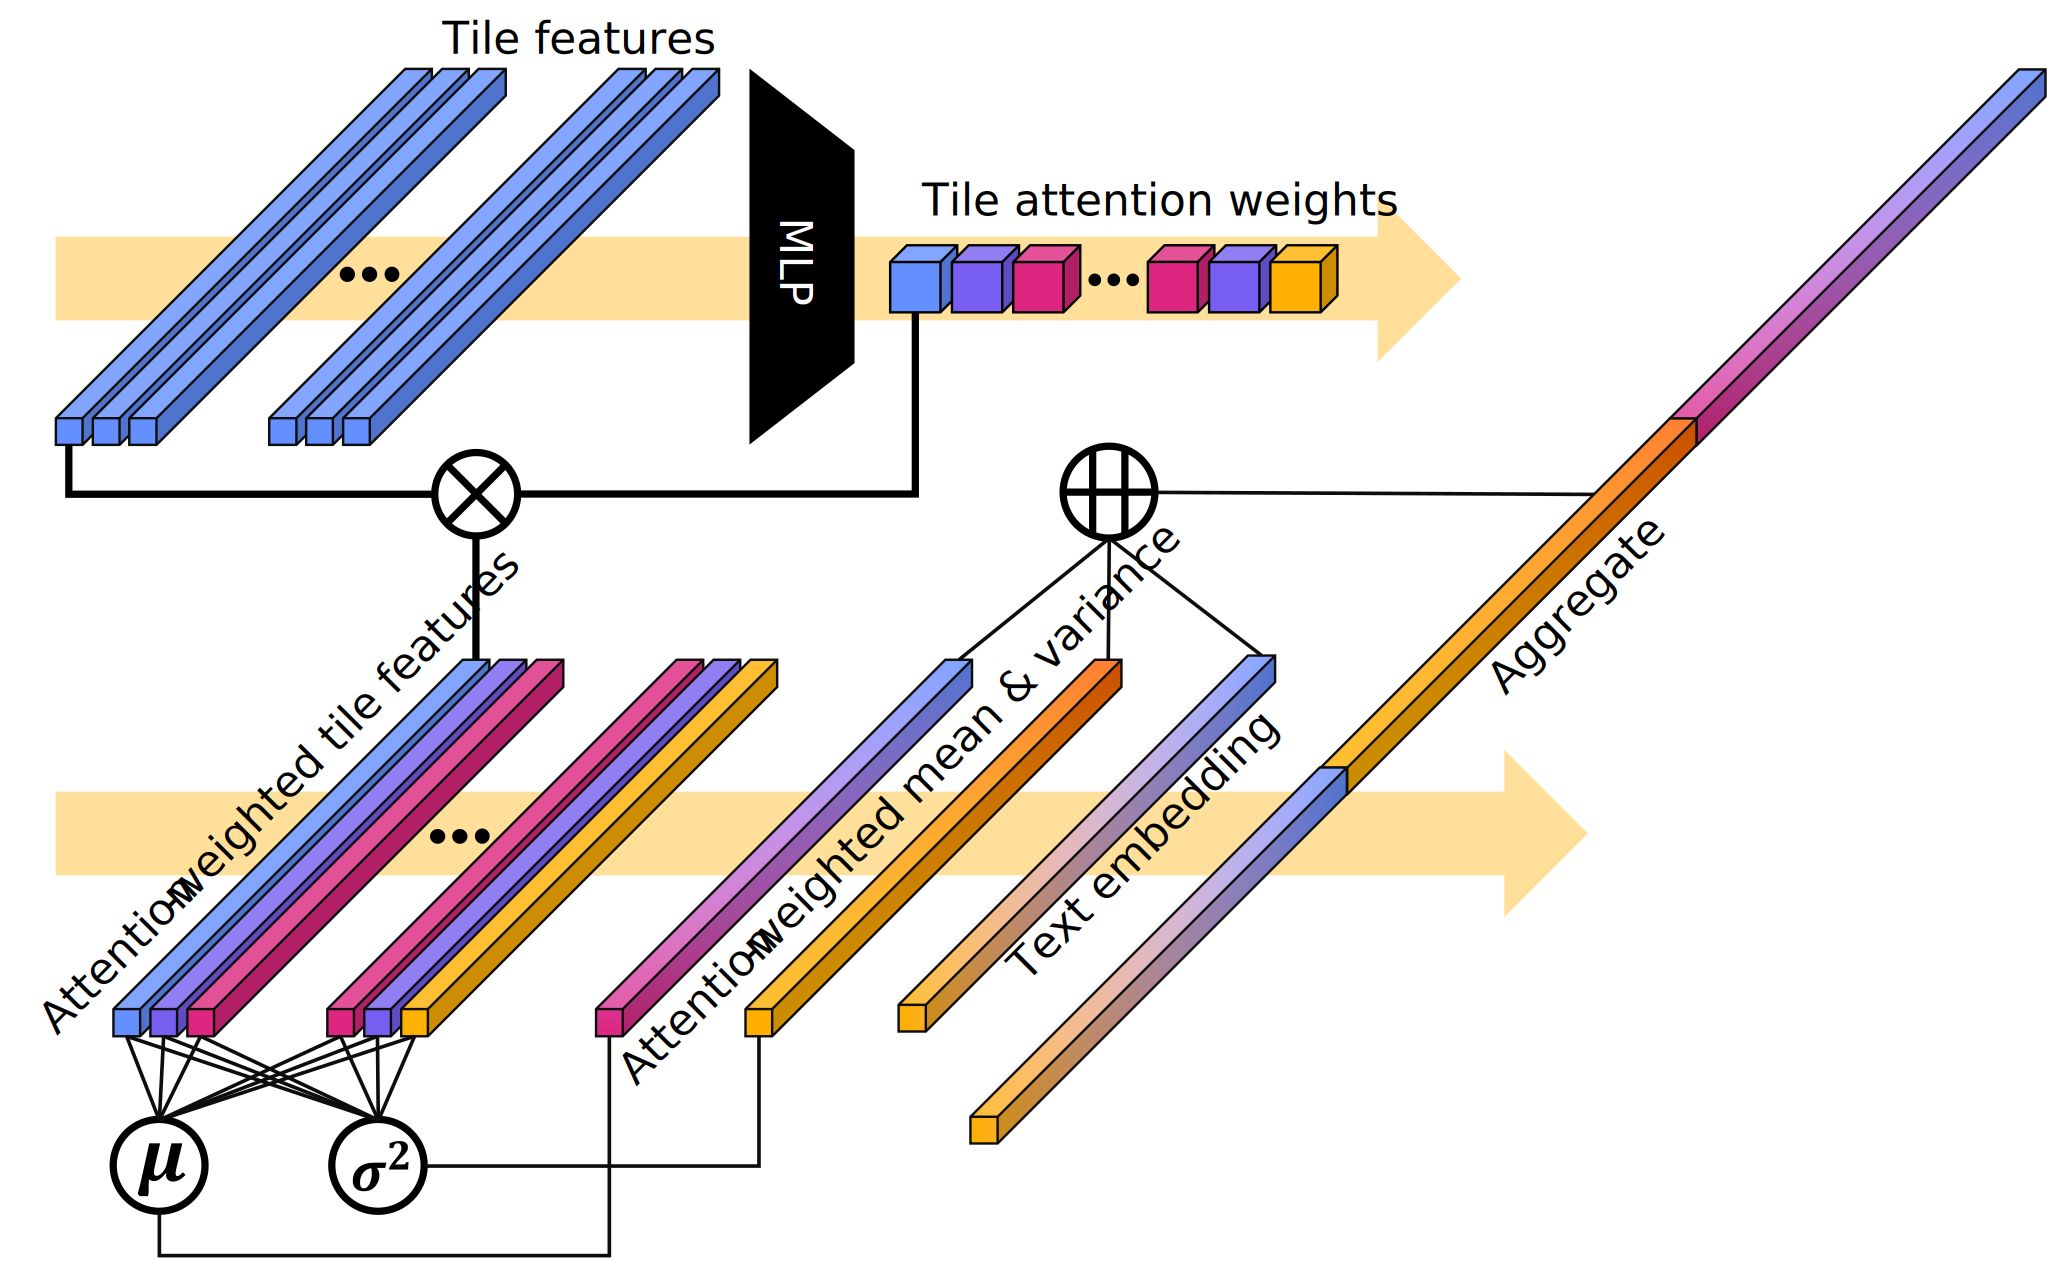
\includegraphics[width=\linewidth]{pediatric-brain-tumours/images/ccmil.png}
    \caption[Clinical Context Multi-Instance Learning aggregator.]{
            Clinical Context Multi-Instance Learning (CCMIL) aggregator.
            Just like in Variance MIL (VarMIL), tile features are presented to a multi-layer perceptron (MLP) to learn attention weights per tile.
            The attention weights are multiplied with their corresponding tile features to get attention-weighted tile features.
            From these, the mean $\mu$ and variance $\sigma^2$ are calculated and concatenated.
            Extending VarMIL, CCMIL further concatenates a text embedding that may contain clinical context of the input image.
            The aggregate is further processed in another MLP for classification.
        }
    \label{fig:CCMIL_aggregator}
\end{figure*}

